\documentclass[12pt,fleqn]{article}
\usepackage{
  amsmath,
  hyperref,
  booktabs,
  geometry,
  graphicx,
  microtype,
  parskip,
}
\usepackage[shortlabels]{enumitem}

\geometry{margin=3cm}

% equation line spacing
\setlength{\jot}{0.5cm}

% meta data
\newcommand{\chapter}{Chapter 7\--8}
\newcommand{\authorname}{Amo DelBello}
\newcommand{\classdescription}{MATH 1350-D2}
\newcommand{\classname}{Introduction to Statistics, Fall 2022}
\newcommand{\assignment}{\chapter\ Take Home Exam}

\newcommand{\problem}[1]{\vspace{5ex}\section*{Problem \##1}}
\newcommand{\thead}[1]{\textnormal{\textbf{#1}}}
\newcommand{\tvspace}{\vspace{.25cm}}

\title{\classdescription\ \\ \classname\ \\ $\ $ \\ \assignment}
\author{\authorname}
\date{\today}


\begin{document}
\maketitle

\problem{1}
The confidence interval is not likely to give a good estimate of the proportion of her listeners who support the legislation because the sample is self selecting.


\problem{2}
We need an estimate of $p$ to determine an adequate sample size. The sample proportion ${\hat{p}}$ is the best point estimate of the population proportion $p$.
\begin{enumerate}
\item When an estimate of $\hat{p}$ is known we use the following formula:
  \begin{align*}
    n &= \frac{[z_{\alpha / 2}]^2 \hat{p} \hat{q}}{E^2}
  \end{align*}
\item When an estimate of $\hat{p}$ is not known we use the following formula (substituting 0.5 for each of the values of $\hat{p}$ and $\hat{q}$):
  \begin{align*}
    n &= \frac{[z_{\alpha / 2}]^2 0.25}{E^2}
  \end{align*}

\end{enumerate}


\problem{3}
\begin{enumerate}
\item If the claim is left-tailed, the critical region is in the extreme left region.
\item If the claim is right-tailed, the critical region is in the extreme right region.
\item For right and left-tailed tests, the symbol used in the alternative hypothesis will determine if the claim is right or left-tailed. If the symbol is $>$, the test is right tailed. If the symbol is $<$, the test is left tailed.
\end{enumerate}

\problem{4}
\begin{tabular}{@{}l p{6cm}  p{6cm} @{}}
  \thead{Test about} & \thead{Distribution} & \thead{Assumptions} \\
  \toprule
  Mean &
  The population is normally distributed or $n > 30$ &
  The sample is a simple random sample \\
  \midrule
  Proportion &
  The conditions for a \textit{binomial distribution} are satisfied &
  The conditions $np \ge 5$ and $nq \ge 5$ are both satisfied and the sample observations are a simple random sample \\
  \midrule
  Variance &
  The population must have a normal distribution &
  The sample is a simple random sample \\
  \bottomrule
\end{tabular}


\problem{5}
In order to use the t distribution to compute the margin of error, the sample size must be $\ge30$ or it must be assumed that the population is normally distributed.


\problem{6}
In addition to an estimate of the value of the population mean, a confidence interval also gives us an indication of how accurate that estimate is.


\problem{7}
\begin{enumerate}[label=\alph*.]


\item Are the female bears older than the male bears?
\begin{align*}
  H_0: \mu_1 &= \mu_2 \\
  H_1: \mu_1 &> \mu_2 \\
  \text{Test Statistic, t:} &= 1.255 \\
  \text{P-Value:} &= 0.108
\end{align*}
Because the P-Value is greater than or equal to the significance level of $\alpha = 0.05$, we fail to reject the null hypothesis. We cannot support the claim that the female bears are older than the male bears.
\begin{figure}[ht]
  \centering
  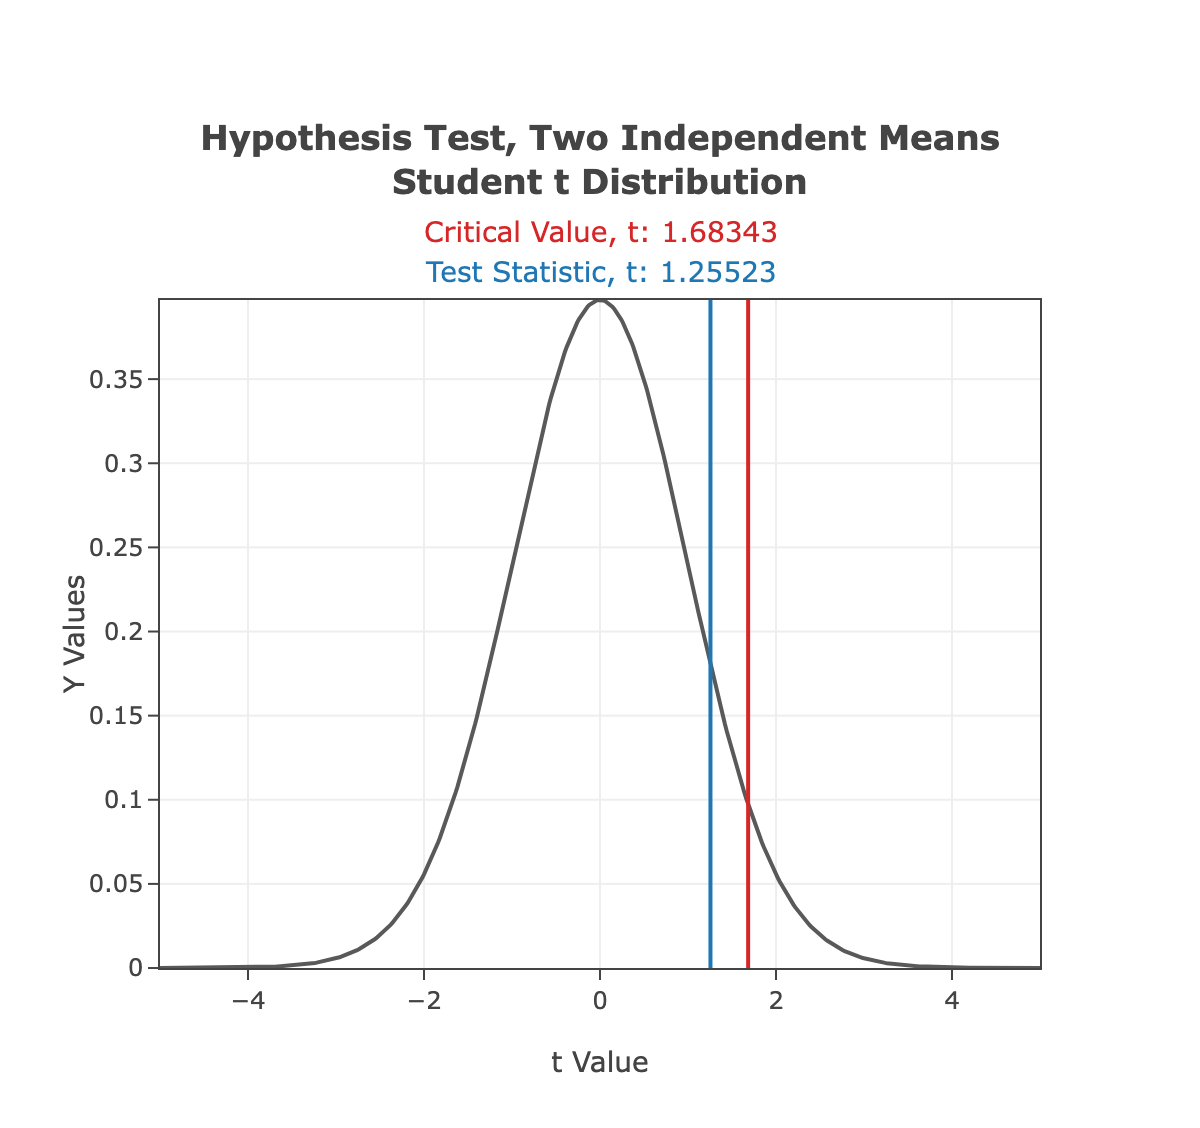
\includegraphics[width=12cm]{assets/bears.png}
\end{figure}


\item Are the female head lengths different from those of males?
\begin{align*}
  H_0: \mu_1 &= \mu_2 \\
  H_1: \mu_1 &\ne \mu_2 \\
  \text{Test Statistic, t:} &= -1.392 \\
  \text{P-Value:} &= 0.171
\end{align*}
95\% Confidence Interval:
\begin{align*}
  -1.911 < \mu_1 - \mu_2 < 0.349
\end{align*}
Because the confidence interval contains zero we cannot support the claim that the head lengths are different.
\begin{figure}[ht]
  \centering
  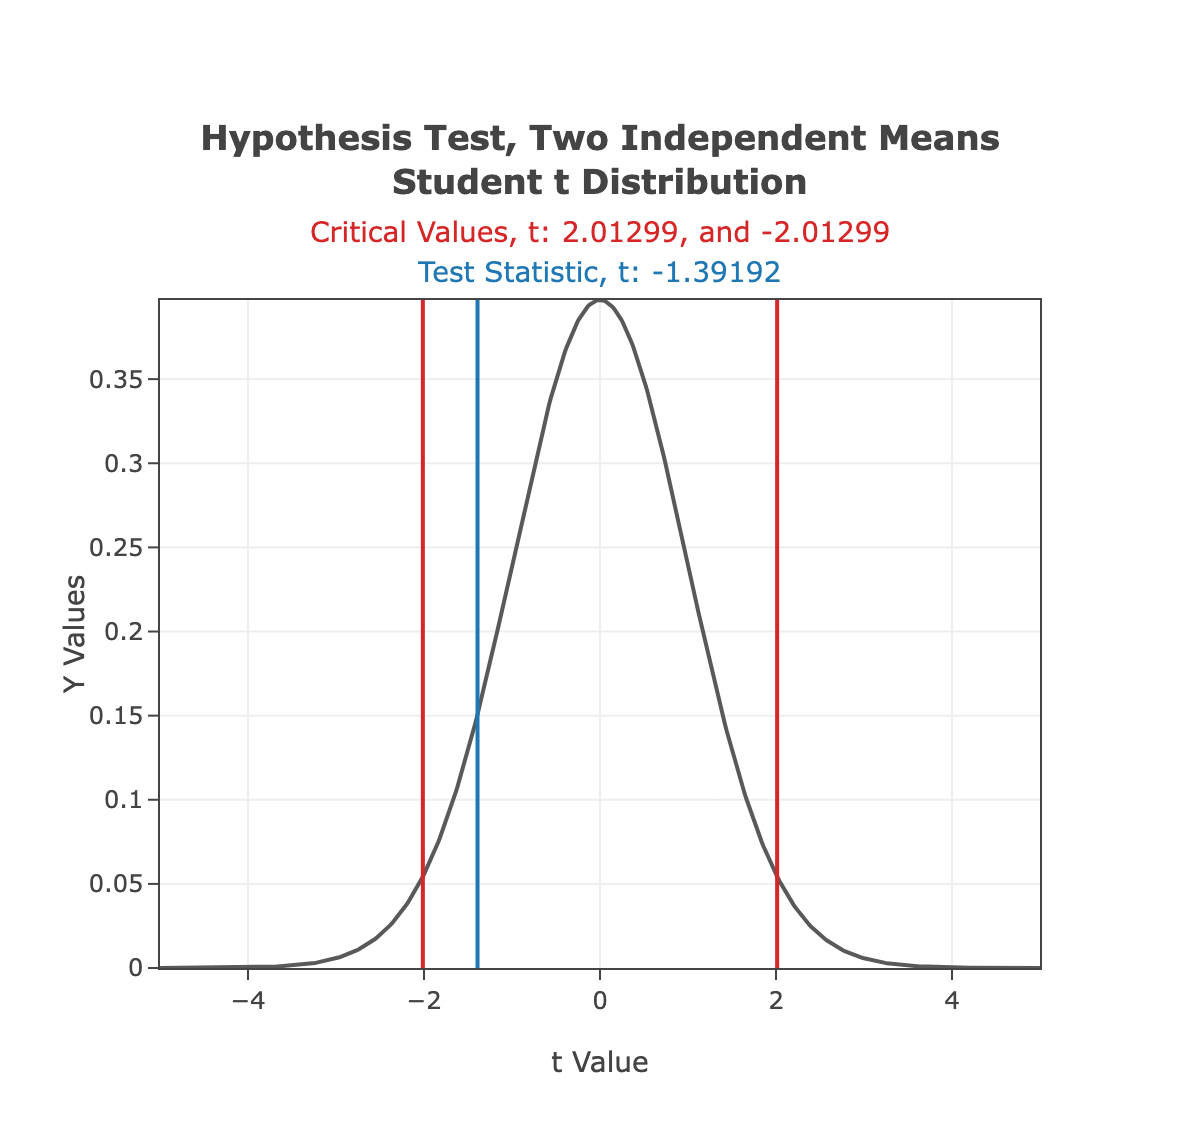
\includegraphics[width=12cm]{assets/head-lengths.png}
\end{figure}


\item Are the standard deviation in weights the same for male and female bears?
\begin{align*}
  H_0: \sigma_1 &= \sigma_2 \\
  H_1: \sigma_1 &\ne \sigma_2 \\
\end{align*}
95\% Confidence Interval:
\begin{align*}
  0.457 < \sigma_1/\sigma_2 < 1.05
\end{align*}
Because the confidence interval does not contain zero we can support the claim that the standard deviations in weight between the male and female bears are not the same.


\item What are we not accounting for?

The only thing I can think of is that we are not making sure that the sample of the female bears is normally distributed because we have a sample size of only 19.

\end{enumerate}
\end{document}
